\documentclass{standalone}
\usepackage{tikz}
\usetikzlibrary{patterns, positioning}


\begin{document}
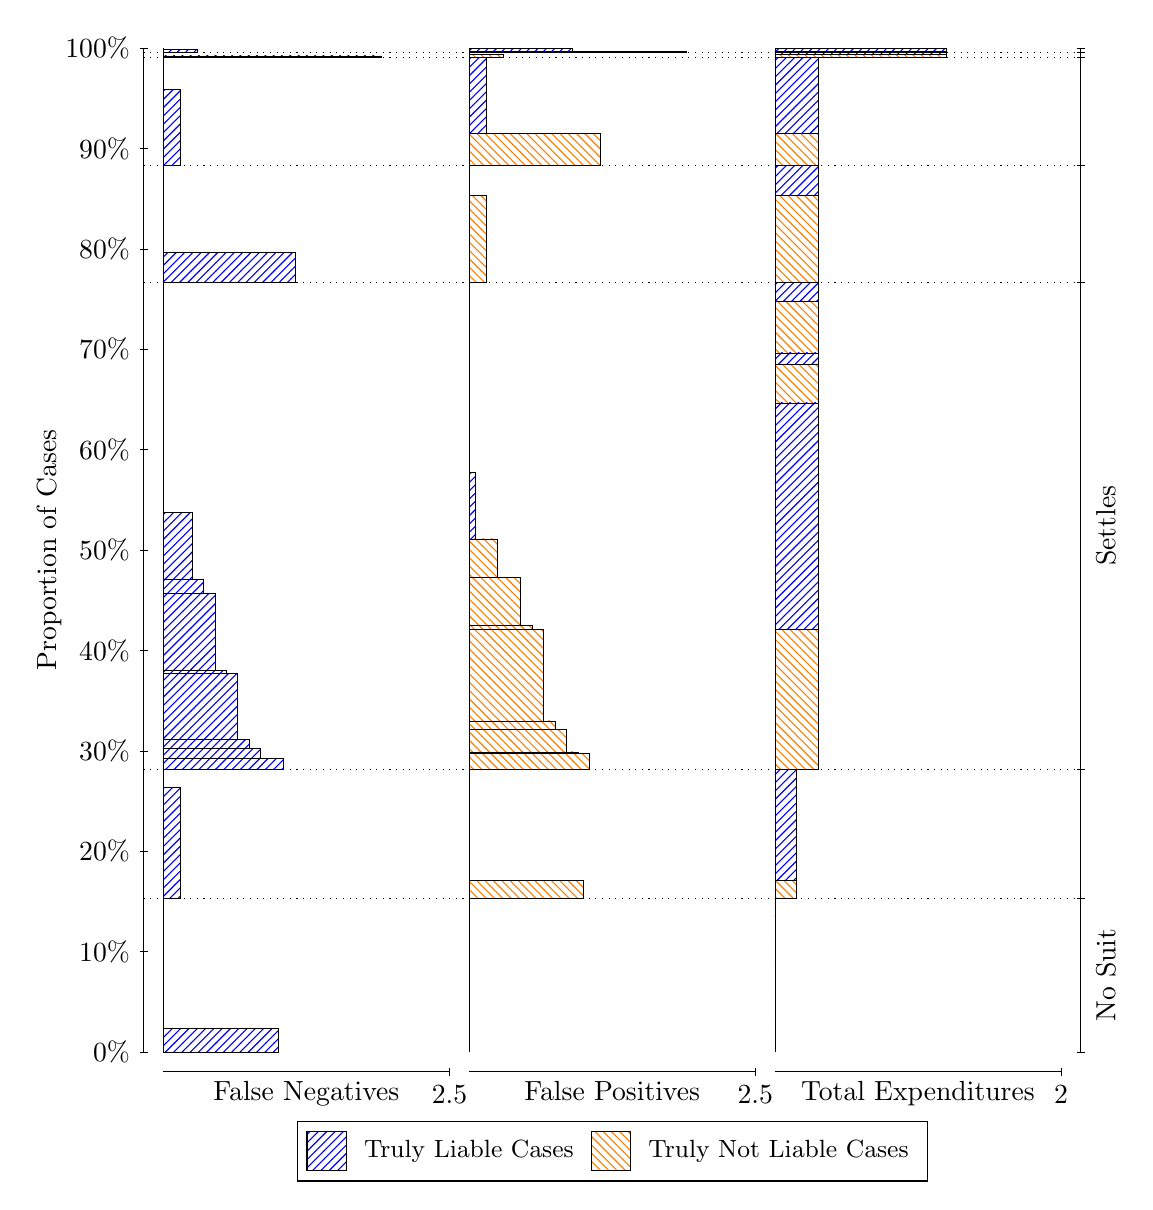
\begin{tikzpicture}
\draw[black, very thin] (1.5,1.75) -- (1.5,14.5);
\node[rotate=90, text=black, anchor=center] at (0.3, 8.125) {Proportion of Cases};
\draw[black, very thin] (1.45,1.75) -- (1.55,1.75);
\node[text=black, anchor=east] at (1.45, 1.75) {0\%};
\draw[black, very thin] (1.45,3.025) -- (1.55,3.025);
\node[text=black, anchor=east] at (1.45, 3.025) {10\%};
\draw[black, very thin] (1.45,4.3) -- (1.55,4.3);
\node[text=black, anchor=east] at (1.45, 4.3) {20\%};
\draw[black, very thin] (1.45,5.575) -- (1.55,5.575);
\node[text=black, anchor=east] at (1.45, 5.575) {30\%};
\draw[black, very thin] (1.45,6.85) -- (1.55,6.85);
\node[text=black, anchor=east] at (1.45, 6.85) {40\%};
\draw[black, very thin] (1.45,8.125) -- (1.55,8.125);
\node[text=black, anchor=east] at (1.45, 8.125) {50\%};
\draw[black, very thin] (1.45,9.4) -- (1.55,9.4);
\node[text=black, anchor=east] at (1.45, 9.4) {60\%};
\draw[black, very thin] (1.45,10.675) -- (1.55,10.675);
\node[text=black, anchor=east] at (1.45, 10.675) {70\%};
\draw[black, very thin] (1.45,11.95) -- (1.55,11.95);
\node[text=black, anchor=east] at (1.45, 11.95) {80\%};
\draw[black, very thin] (1.45,13.225) -- (1.55,13.225);
\node[text=black, anchor=east] at (1.45, 13.225) {90\%};
\draw[black, very thin] (1.45,14.5) -- (1.55,14.5);
\node[text=black, anchor=east] at (1.45, 14.5) {100\%};

\draw[black, very thin] (13.4,1.75) -- (13.4,14.5);
\draw[black, very thin] (13.35,1.75) -- (13.45,1.75);
\node[anchor=west] at (13.35, 1.75) {};
\draw[black, very thin] (13.35,3.7029) -- (13.45,3.7029);
\node[anchor=west] at (13.35, 3.7029) {};
\draw[black, very thin] (13.35,5.3403) -- (13.45,5.3403);
\node[anchor=west] at (13.35, 5.3403) {};
\draw[black, very thin] (13.35,11.524) -- (13.45,11.524);
\node[anchor=west] at (13.35, 11.524) {};
\draw[black, very thin] (13.35,13.007) -- (13.45,13.007);
\node[anchor=west] at (13.35, 13.007) {};
\draw[black, very thin] (13.35,14.381) -- (13.45,14.381);
\node[anchor=west] at (13.35, 14.381) {};
\draw[black, very thin] (13.35,14.441) -- (13.45,14.441);
\node[anchor=west] at (13.35, 14.441) {};
\draw[black, very thin] (13.35,14.5) -- (13.45,14.5);
\node[anchor=west] at (13.35, 14.5) {};

\draw[black, very thin, pattern color=blue, pattern=north east lines] (1.75,1.75) rectangle (3.2033,2.0517);
\draw[black, very thin, pattern color=orange, pattern=north west lines] (1.75,2.0517) rectangle (1.75,3.7029);
\draw[black, very thin, pattern color=blue, pattern=north east lines] (1.75,3.7029) rectangle (1.968,5.1114);
\draw[black, very thin, pattern color=orange, pattern=north west lines] (1.75,5.1114) rectangle (1.75,5.3403);
\draw[black, very thin, pattern color=blue, pattern=north east lines] (1.75,5.3403) rectangle (3.276,5.4829);
\draw[black, very thin, pattern color=blue, pattern=north east lines] (1.75,5.4829) rectangle (2.9853,5.6074);
\draw[black, very thin, pattern color=blue, pattern=north east lines] (1.75,5.6074) rectangle (2.84,5.7191);
\draw[black, very thin, pattern color=blue, pattern=north east lines] (1.75,5.7191) rectangle (2.6947,6.5548);
\draw[black, very thin, pattern color=blue, pattern=north east lines] (1.75,6.5548) rectangle (2.5493,6.5923);
\draw[black, very thin, pattern color=blue, pattern=north east lines] (1.75,6.5923) rectangle (2.404,7.576);
\draw[black, very thin, pattern color=blue, pattern=north east lines] (1.75,7.576) rectangle (2.2587,7.753);
\draw[black, very thin, pattern color=blue, pattern=north east lines] (1.75,7.753) rectangle (2.1133,8.5991);
\draw[black, very thin, pattern color=orange, pattern=north west lines] (1.75,8.5991) rectangle (1.75,11.524);
\draw[black, very thin, pattern color=blue, pattern=north east lines] (1.75,11.524) rectangle (3.4213,11.902);
\draw[black, very thin, pattern color=orange, pattern=north west lines] (1.75,11.902) rectangle (1.75,13.007);
\draw[black, very thin, pattern color=blue, pattern=north east lines] (1.75,13.007) rectangle (1.968,13.976);
\draw[black, very thin, pattern color=orange, pattern=north west lines] (1.75,13.976) rectangle (1.75,14.381);
\draw[black, very thin, pattern color=blue, pattern=north east lines] (1.75,14.381) rectangle (4.5113,14.399);
\draw[black, very thin, pattern color=orange, pattern=north west lines] (1.75,14.399) rectangle (1.75,14.441);
\draw[black, very thin, pattern color=blue, pattern=north east lines] (1.75,14.441) rectangle (2.186,14.482);
\draw[black, very thin, pattern color=orange, pattern=north west lines] (1.75,14.482) rectangle (1.75,14.5);
\draw[black, very thin, pattern color=orange, pattern=north west lines] (5.6333,1.75) rectangle (5.6333,3.4012);
\draw[black, very thin, pattern color=blue, pattern=north east lines] (5.6333,3.4012) rectangle (5.6333,3.7029);
\draw[black, very thin, pattern color=orange, pattern=north west lines] (5.6333,3.7029) rectangle (7.0867,3.9318);
\draw[black, very thin, pattern color=blue, pattern=north east lines] (5.6333,3.9318) rectangle (5.6333,5.3403);
\draw[black, very thin, pattern color=orange, pattern=north west lines] (5.6333,5.3403) rectangle (7.1593,5.5377);
\draw[black, very thin, pattern color=orange, pattern=north west lines] (5.6333,5.5377) rectangle (7.014,5.5619);
\draw[black, very thin, pattern color=orange, pattern=north west lines] (5.6333,5.5619) rectangle (6.8687,5.8457);
\draw[black, very thin, pattern color=orange, pattern=north west lines] (5.6333,5.8457) rectangle (6.7233,5.9549);
\draw[black, very thin, pattern color=orange, pattern=north west lines] (5.6333,5.9549) rectangle (6.578,7.1139);
\draw[black, very thin, pattern color=orange, pattern=north west lines] (5.6333,7.1139) rectangle (6.4327,7.1634);
\draw[black, very thin, pattern color=orange, pattern=north west lines] (5.6333,7.1634) rectangle (6.2873,7.7735);
\draw[black, very thin, pattern color=orange, pattern=north west lines] (5.6333,7.7735) rectangle (5.9967,8.265);
\draw[black, very thin, pattern color=blue, pattern=north east lines] (5.6333,8.265) rectangle (5.706,9.1112);
\draw[black, very thin, pattern color=blue, pattern=north east lines] (5.6333,9.1112) rectangle (5.6333,11.524);
\draw[black, very thin, pattern color=orange, pattern=north west lines] (5.6333,11.524) rectangle (5.8513,12.629);
\draw[black, very thin, pattern color=blue, pattern=north east lines] (5.6333,12.629) rectangle (5.6333,13.007);
\draw[black, very thin, pattern color=orange, pattern=north west lines] (5.6333,13.007) rectangle (7.3047,13.412);
\draw[black, very thin, pattern color=blue, pattern=north east lines] (5.6333,13.412) rectangle (5.8513,14.381);
\draw[black, very thin, pattern color=orange, pattern=north west lines] (5.6333,14.381) rectangle (6.0693,14.423);
\draw[black, very thin, pattern color=blue, pattern=north east lines] (5.6333,14.423) rectangle (5.6333,14.441);
\draw[black, very thin, pattern color=orange, pattern=north west lines] (5.6333,14.441) rectangle (8.3947,14.459);
\draw[black, very thin, pattern color=blue, pattern=north east lines] (5.6333,14.459) rectangle (6.9413,14.5);
\draw[black, very thin, pattern color=orange, pattern=north west lines] (9.5167,1.75) rectangle (9.5167,3.4012);
\draw[black, very thin, pattern color=blue, pattern=north east lines] (9.5167,3.4012) rectangle (9.5167,3.7029);
\draw[black, very thin, pattern color=orange, pattern=north west lines] (9.5167,3.7029) rectangle (9.7892,3.9318);
\draw[black, very thin, pattern color=blue, pattern=north east lines] (9.5167,3.9318) rectangle (9.7892,5.3403);
\draw[black, very thin, pattern color=orange, pattern=north west lines] (9.5167,5.3403) rectangle (10.062,7.1139);
\draw[black, very thin, pattern color=blue, pattern=north east lines] (9.5167,7.1139) rectangle (10.062,9.9939);
\draw[black, very thin, pattern color=orange, pattern=north west lines] (9.5167,9.9939) rectangle (10.062,10.485);
\draw[black, very thin, pattern color=blue, pattern=north east lines] (9.5167,10.485) rectangle (10.062,10.628);
\draw[black, very thin, pattern color=orange, pattern=north west lines] (9.5167,10.628) rectangle (10.062,11.288);
\draw[black, very thin, pattern color=blue, pattern=north east lines] (9.5167,11.288) rectangle (10.062,11.524);
\draw[black, very thin, pattern color=orange, pattern=north west lines] (9.5167,11.524) rectangle (10.062,12.629);
\draw[black, very thin, pattern color=blue, pattern=north east lines] (9.5167,12.629) rectangle (10.062,13.007);
\draw[black, very thin, pattern color=orange, pattern=north west lines] (9.5167,13.007) rectangle (10.062,13.412);
\draw[black, very thin, pattern color=blue, pattern=north east lines] (9.5167,13.412) rectangle (10.062,14.381);
\draw[black, very thin, pattern color=orange, pattern=north west lines] (9.5167,14.381) rectangle (11.697,14.423);
\draw[black, very thin, pattern color=blue, pattern=north east lines] (9.5167,14.423) rectangle (11.697,14.441);
\draw[black, very thin, pattern color=orange, pattern=north west lines] (9.5167,14.441) rectangle (11.697,14.459);
\draw[black, very thin, pattern color=blue, pattern=north east lines] (9.5167,14.459) rectangle (11.697,14.5);
\draw[black, dotted] (1.5,3.7029) -- (13.4,3.7029);
\draw[black, dotted] (1.5,5.3403) -- (13.4,5.3403);
\draw[black, dotted] (1.5,11.524) -- (13.4,11.524);
\draw[black, dotted] (1.5,13.007) -- (13.4,13.007);
\draw[black, dotted] (1.5,14.381) -- (13.4,14.381);
\draw[black, dotted] (1.5,14.441) -- (13.4,14.441);
\draw[black, very thin] (1.75,1.5) -- (5.3833,1.5);
\node[text=black, anchor=north] at (3.5667, 1.5) {False Negatives};
\draw[black, very thin] (5.3833,1.45) -- (5.3833,1.55);
\node[text=black, anchor=north] at (5.3833, 1.45) {2.5};

\draw[black, very thin] (5.6333,1.5) -- (9.2667,1.5);
\node[text=black, anchor=north] at (7.45, 1.5) {False Positives};
\draw[black, very thin] (9.2667,1.45) -- (9.2667,1.55);
\node[text=black, anchor=north] at (9.2667, 1.45) {2.5};

\draw[black, very thin] (9.5167,1.5) -- (13.15,1.5);
\node[text=black, anchor=north] at (11.333, 1.5) {Total Expenditures};
\draw[black, very thin] (13.15,1.45) -- (13.15,1.55);
\node[text=black, anchor=north] at (13.15, 1.45) {2};

\node[text=black, centered, rotate=90] at (13.72, 2.7265) {No Suit};

\node[text=black, centered, rotate=90] at (13.72, 8.4321) {Settles};





\draw (7.449999999999999,1.5) node[draw=none] (baseCoordinate) {};
\begin{scope}[align=center]
        \matrix[scale=0.5, draw=black, below=0.5cm of baseCoordinate, nodes={draw}, column sep=0.1cm]{
            \node[rectangle, draw, minimum width=0.5cm, minimum height=0.5cm, pattern color=blue, pattern=north east lines] {}; &
            \node[draw=none, font=\small, text=black] (B) {Truly Liable Cases}; &
            \node[rectangle, draw, minimum width=0.5cm, minimum height=0.5cm, pattern color=orange, pattern=north west lines] {}; &
            \node[draw=none, font=\small, text=black] (B) {Truly Not Liable Cases}; \\
            };
\end{scope}

\end{tikzpicture}
\end{document}